\chapter{Periodic Structure of Crystalline Solids}
\section{Condensed matter}
To introduce you to condensed matter, we will define some solid structures:
\dfn{Solid structures}{
	\begin{itemize}
		\setlength\itemsep{0pt}
		\item Crystalline solids - metals
		\item Amorphous solids - glass
		\item Liquid crystals
		\item Quasi Crystals
		\item Polymers
	\end{itemize}
}

\section{Crystals} \label{sec:crystals}
\dfn{Crystal}{A crystal is a lattice and a basis, which in essence is a \textbf{periodic arrangement of atoms}.}
For now, lets define a lattice as follows:
\dfn{Lattice (1)}{A lattice is an infinite array of identical points, arranged such that each point sees the other points in an identical way.}
We can define a basis in the following way:
\dfn{Basis}{A basis is a structural unit representation by lattice points. The units in which it can be defined are i.e.:
	\begin{itemize}
		\setlength\itemsep{0pt}
		\item Atoms
		\item Molecules
		\item Group of atoms
	\end{itemize}
}

Let's look at some lattices, depicted in figure \ref{fig:lattices}. The parameter $a$ is the lattice parameter.\par
\begin{figure}[h]
	\centering
	\tcbsidebyside[sidebyside adapt=left, blanker, sidebyside gap=1cm,
               sidebyside align=top seam]{\hspace{150pt}\textit{1D:}}{
	\begin{tikzpicture}
		\filldraw [black]	(0,0.35) circle (2pt)
							(1,0.35) circle (2pt)
							(2,0.35) circle (2pt)
							(3,0.35) circle (2pt)
							(4,0.35) circle (2pt)
							(5,0.35) circle (2pt)
							(6,0.35) circle (2pt);
		\draw [<->, black, thick]	(1, 0) to ["a"] (2, 0);
	\end{tikzpicture}}

	\vspace{10pt}

	\tcbsidebyside[sidebyside adapt=left, blanker, sidebyside gap=1cm,
               sidebyside align=top seam]{\hspace{150pt}\textit{2D:}}{
	\begin{tikzpicture}
		\filldraw [black]	(0,0) circle (2pt)
							(1,0) circle (2pt)
							(2,0) circle (2pt)
							(3,0) circle (2pt)
							(4,0) circle (2pt)
							(5,0) circle (2pt)
							(6,0) circle (2pt)
							(0,1) circle (2pt)
							(1,1) circle (2pt)
							(2,1) circle (2pt)
							(3,1) circle (2pt)
							(4,1) circle (2pt)
							(5,1) circle (2pt)
							(6,1) circle (2pt)
							(0,2) circle (2pt)
							(1,2) circle (2pt)
							(2,2) circle (2pt)
							(3,2) circle (2pt)
							(4,2) circle (2pt)
							(5,2) circle (2pt)
							(6,2) circle (2pt);
		\draw [<->, black, thick]	(1, 0.35) to ["a"] (2, 0.35);
		\draw [<->, black, thick]	(0.35, 0) to ["a"] (0.35, 1);
	\end{tikzpicture}}

	\vspace{10pt}

	\tcbsidebyside[sidebyside adapt=left, blanker, sidebyside gap=1cm,
               sidebyside align=top seam]{\hspace{150pt}\textit{3D:}}{
	\begin{tikzpicture}
		%	Bottom front
		\draw [*-, black]	(0, 0) to (1, 0);
		\filldraw [black]	(1, 0) circle (2pt);
		\draw [-*, black]	(1, 0) to (2, 0);

		%	Top front
		\draw [*-, black]	(0, 1) to (1, 1);
		\filldraw [black]	(1, 1) circle (2pt);
		\draw [-*, black]	(1, 1) to (2, 1);

		%	Horzontal front
		\draw[-, black]	(0.1, 0) to (0.1, 1)
							(1, 0) to (1, 1)
							(1.9, 0) to (1.9, 1);

		%	Top oblique
		\draw[-*, black]	(0.1, 1) to (0.65, 1.5);
		\draw[-*, black]	(1, 1) to (1.55, 1.5);
		\draw[-*, black]	(1.9, 1) to (2.45, 1.5);

		%	Side right
		\draw[-*, black]	(2.4, 1.5) to (2.4, 0.4);
		\draw[-, black]	(1.9, 0) to (2.4, 0.5);

		%	Top back
		\draw[-, black]	(0.6, 1.45) to (2.4, 1.45);

		%	Inside
		\draw[dotted, black]	(0.1, 0) to (0.6, 0.5)
								(0.6, 0.5) to (2.4, 0.5)
								(0.6, 0.5) to (0.6, 1.5)
								(1.5, 0.5) to (1, 0)
								(1.5, 1.5) to (1.5, 0.5);
		\filldraw[black]	(0.6, 0.5) circle (1pt)
							(1.5, 0.5) circle (1pt);

 		\draw [<->, black, thick]	(1, -0.3) to node [below] {a} (1.9, -0.3);
 		\draw [<->, black, thick]	(2.7, 0.5) to node [right] {a} (2.7, 1.5);
 		\draw [<->, black, thick]	(2.1, -0.1) to node [right=1.2mm, below=0.01mm] {a} (2.6, 0.4);
	\end{tikzpicture}}
	\caption{Lattices in different dimensions}
	\label{fig:lattices}
\end{figure}

As we can probably see, we can always define a some minimal set of vectors that describe the lattice. That means we can indeed go to each lattice point by taking a linear combination of these vectors. An example is given in figure \ref{fig:example_lattice}. \textit{More examples can be found in the slides.} More on lattice vectors in \ref{sec:lattice_vectors}.
\ex{Graphene}{
To show what a lattice is and what it isn't this example is given, see also figure \ref{fig:graphene_lattices}. As we know, graphene has a honeycomb lattice. That's why we call it a honneycomb crystal. But the lattice we can define is called a triangular lattice. Why?\\ \newline
By the definition of a lattice, we must have the same surrounding for every lattice point. This is not the case if we take one atom as basis. Therefore we take a set of two atoms to form the basis and define the lattice point as the center. This results in an equivalent surrounding for every basis structure. \\ \newline
Later on we will define a unit cell (section \ref{sec:unit_cell}) and a conventional unit cell (section \ref{sec:conv_unit_cell}) for this lattice. \todo{Add these to the pdf}
}
\begin{figure}[h]
	\centering
	\includegraphics[width=\textwidth/2]{./graphene_lattice}
	\caption{The graphene crystal}
	\label{fig:graphene_lattices}
\end{figure}

\section{Lattice vectors} \label{sec:lattice_vectors}
As already touched upon at section \ref{sec:crystals}, we can define a set of lattice vectors. To construct these we first define an origin O:
\begin{equation}
	O = \vec{0}
\end{equation}
Then we will define the lattice points in function of the PLV \textit{(Primitive Lattice Vectors)}.
\begin{align}
	\vec{a} &= PLV \\
	n_i &\in \bbZ \\
	A &= [\vec{a}_1, \vec{a}_2(, \vec{a}_3)]^T \\
	1D &: \qquad \vec{R} = n_1 \cdot \vec{a} \\
	2D &: \qquad \vec{R} = [n_1, n_2] \cdot A \\
	3D &: \qquad \vec{R} = [n_1, n_2, n_3] \cdot A
\end{align}

We can understand that a lattice must be defined unambiguous, therefore the definition of a lattice can be defined as:
\dfn{Lattice (2)}{A lattice is a set of points defined by Primitive Lattice Vectors (PLV).}
Visually we can represent these vectors as can be seen in figure \ref{fig:example_1Dlattice} and figure \ref{fig:example_lattice}. We can also conclude that \textit{PLV}s are not unique, one can also show that this is true for 3D. These are indeed \textit{PLV}s because one can reach all lattice points.
\begin{figure}[h]
	\centering
	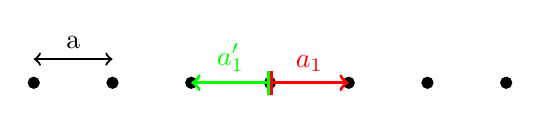
\begin{tikzpicture}
		\filldraw [black]	(0, 0) circle (2pt)
							(1, 0) circle (2pt)
							(2, 0) circle (2pt)
							(3, 0) circle (2pt)
							(4, 0) circle (2pt)
							(5, 0) circle (2pt)
							(6, 0) circle (2pt);
		\draw [|->, red, very thick]	(3, 0) to node [above]{$a_1$} (4, 0);
		\draw [|->, green, very thick]	(3, 0) to node [above]{$a_1'$} (2, 0);

		\draw [<->, black, thick]	(0, 0.3) to node [above]{a} (1, 0.3);
	\end{tikzpicture}
	\caption{An example set of lattice vectors in 1D}
	\label{fig:example_1Dlattice}
\end{figure}
\begin{figure}[h]
	\centering
	\begin{tikzpicture}
		\filldraw [black]	(0,0) circle (2pt)
							(1,0) circle (2pt)
							(2,0) circle (2pt)
							(3,0) circle (2pt)
							(4,0) circle (2pt)
							(5,0) circle (2pt)
							(6,0) circle (2pt)
							(0,1) circle (2pt)
							(1,1) circle (2pt)
							(2,1) circle (2pt)
							(3,1) circle (2pt)
							(4,1) circle (2pt)
							(5,1) circle (2pt)
							(6,1) circle (2pt)
							(0,2) circle (2pt)
							(1,2) circle (2pt)
							(2,2) circle (2pt)
							(3,2) circle (2pt)
							(4,2) circle (2pt)
							(5,2) circle (2pt)
							(6,2) circle (2pt);
		\draw [<->, black, thick]	(1, 1.35) to ["a"] (2, 1.35);
		\draw [<->, black, thick]	(2.35, 0) to node [right]{a} (2.35, 1);

		\draw [|->, red, very thick]	(0, 0) to node [left]{$a_1$} (0, 1);
		\draw [|->, green, very thick]	(0, 0) to node [below]{$a_2$}(1, 0);

		\draw [|->, red, very thick]	(4, 0) to node [left]{$a_1'$} (4, 1);
		\draw [|->, green, very thick]	(4, 0) to node [below]{$a_2'$}(5, 1);
	\end{tikzpicture}
	\caption{An example set of lattice vectors in 2D}
	\label{fig:example_lattice}
\end{figure}

\section{Unit cell} \label{sec:unit_cell}
\dfn{Unit cell}{A unit cell is a region of space such taht when translated through the entire space by means of lattice vecotrs, reproduces the lattice without any overlaps or voids.}
The definition of a unit cell is illustrated in figure \ref{fig:unit_cell}
\begin{figure}[h]
	\centering
	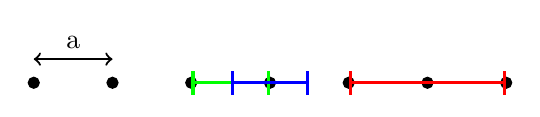
\begin{tikzpicture}
		\filldraw [black]	(0,0) circle (2pt)
							(1,0) circle (2pt)
							(2,0) circle (2pt)
							(3,0) circle (2pt)
							(4,0) circle (2pt)
							(5,0) circle (2pt)
							(6,0) circle (2pt);

		\draw [<->, black , thick]	(0, 0.3) to node [above]{a} (1, 0.3);

		\draw [|-|, green , very thick]	(2, 0) to (3, 0);
		\draw [|-|, red , very thick]	(4, 0) to (6, 0);
		\draw [|-|, blue , very thick]	(2.5, 0) to (3.5, 0);
	\end{tikzpicture}
	\caption{Several 1D unit cells}
	\label{fig:unit_cell}
\end{figure}

\section{Primitive unit cell} \label{sec:prim_unit_cell}
\dfn{Primitive unit cell}{A Primitive Unit Cell (PUC) is a unit cell that contains only one lattice parameter. By this is meant that when for example a cube is a primitive unit cell, each point counts as $\frac{1}{8}$, therefore the cube only has 1 lattice point.}

We then see that:
\begin{itemize}
	\item 1D: line spanned by \textit{PLV} $\vec{a} \Rightarrow$ the line of the \textit{PUC} $= \norm{\vec{a}}$.
	\item 2D: area spanned by \textit{PLV} $\vec{a}_1, \vec{a}_2 \Rightarrow$ the area of the \textit{PUC} $= \norm{\vec{a}_1 \times \vec{a}_2}$.
	\item 3D: volume spanned by \textit{PLV} $\vec{a}_1, \vec{a}_2, \vec{a}_3 \Rightarrow$ the volume of the \textit{PUC} $= \vec{a}_1 \cdot \vec{a}_2 \times \vec{a}_3$.
\end{itemize}

\section{Conventional unit cell} \label{sec:conv_unit_cell}
\dfn{Convetional unit cell}{A convenctional unit cell, a.k.a. a convinient unit cell, is a unit cell that contains mare than 1 lattice point but has perpendicular axis.}

\section{Weigner-Seitz unit cell} \label{sec:weig_cell}
\dfn{Weigner-Seitz unit cell}{A Weigner-Seitz unit cell is a primitive unit cell that has a region of space around a lattice point such that any point around that lattice point is closer to that lattice point as any other lattice point.}

This concept is furhter elaborated below. The correspoding figure for a 2D example is seen in figure \ref{fig:elaboration}.

\begin{enumerate}
	\setlength\itemsep{0pt}
	\item Take any lattice point (green in this case).
	\item Look for the nearest lattice point and draw a line between them (in gray).
	\item Draw the bissecting, perpendicular on this first line (in blue).
	\item Do this for all other nearby lattice points (in cyan).
\end{enumerate}

\begin{figure}[h]
	\centering
	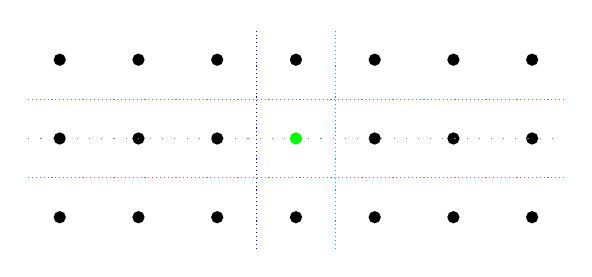
\begin{tikzpicture}
		\filldraw [black]	(0,0) circle (2pt)
							(1,0) circle (2pt)
							(2,0) circle (2pt)
							(3,0) circle (2pt)
							(4,0) circle (2pt)
							(5,0) circle (2pt)
							(6,0) circle (2pt)
							(0,1) circle (2pt)
							(1,1) circle (2pt)
							(2,1) circle (2pt)
							(4,1) circle (2pt)
							(5,1) circle (2pt)
							(6,1) circle (2pt)
							(0,2) circle (2pt)
							(1,2) circle (2pt)
							(2,2) circle (2pt)
							(3,2) circle (2pt)
							(4,2) circle (2pt)
							(5,2) circle (2pt)
							(6,2) circle (2pt);

		\filldraw [green]	(3,1) circle (2pt);

		\draw [loosely dotted, gray] 	(-0.4, 1) to (6.4, 1);

		\draw [densely dotted, blue] 	(2.5, -0.4) to (2.5, 2.4);

		\draw [densely dotted, cyan]	(-0.4, 1.5) to (6.4, 1.5);
		\draw [densely dotted, cyan]	(3.5, -0.4) to (3.5, 2.4);
		\draw [densely dotted, cyan]	(-0.4, 0.5) to (6.4, 0.5);
	\end{tikzpicture}
	\caption{2D example for Weigner-Seitz unit cell}
	\label{fig:elaboration}
\end{figure}
